\graphicspath{{lozano/}}

\section{Relationships Mapping}

Based on the key elements identificated in the past sections, it's proposed the next diagram to representate the system of the competition, where it was drew the parts of the system, and the most significant relationships between them:

\begin{figure}
    \centering
    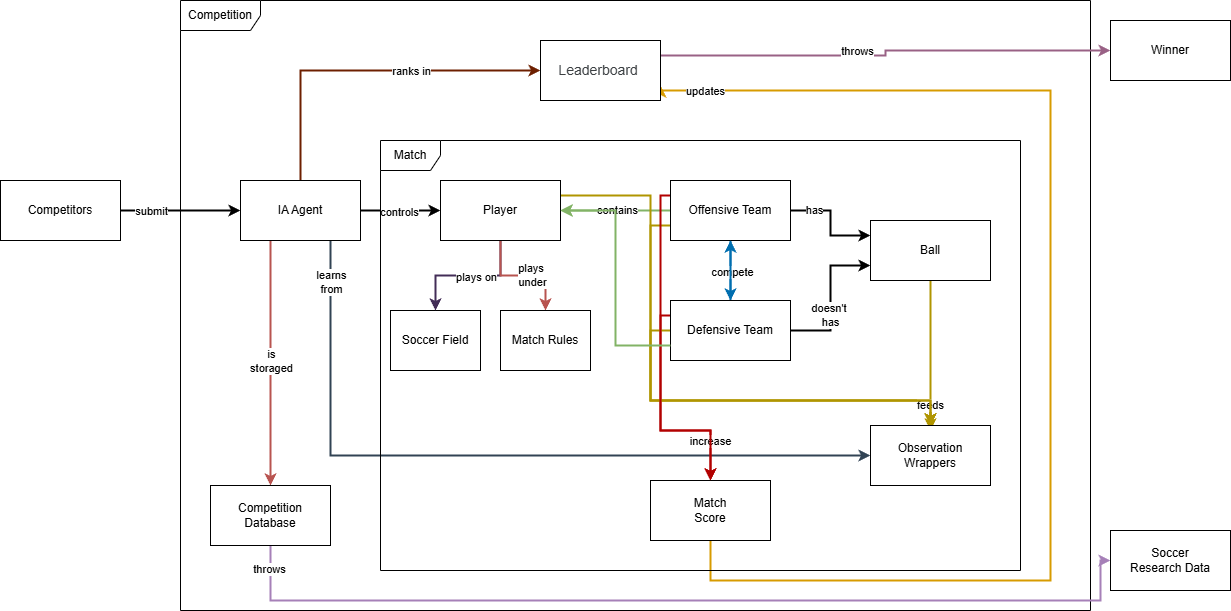
\includegraphics[width=\linewidth]{SystemMapping} 
    \caption{Competition as a system}
\end{figure}

\begin{enumerate}

    \item \textbf{Inputs:}
    \begin{itemize}
        \item Competitors who wants to participate in the competition.
    \end{itemize}

    \item \textbf{Elements of the system:}
    \begin{itemize}
        \item IA Agents submitted by competitors.
        \item Leaderboard that shows the top of the best IA Agents.
        \item Competition Database that stores all of the submissions made by the competitors.
        \item Match sub-system where the IA Agents compete with each other, composed of:
        \begin{itemize}
            \item Players.
            \item Soccer field.
            \item Match rules.
            \item Match score.
            \item Offensive team.
            \item Defensive team.
            \item Ball.
            \item Observation wrappers.
        \end{itemize}
    \end{itemize}

    \item \textbf{Outputs:}
    \begin{itemize}
        \item Winners of the competition.
        \item Soccer Research Data.
    \end{itemize}
\end{enumerate}

\subsection*{System Flow}
\begin{itemize}
\item The system recieves competitors who submit their IA Agent to participate, having two processes with it: the IA agent is stored on the Database of the competition, and the IA agent is tested in a match against itself to test if it works. The competitor can upload up to five agents per day.

\item If it doesn't pass the test, it will be returned as error. Otherwise, it is asignated with a base $\mu$ that represents the estimated skill of the agent, and a $\sigma$ that represents the uncertainty of that estimate, and will decrease everytime that the agent plays.

\item During the competition, the IA Agent with similar $\mu$ will play matches against each other. The winner increase its $\mu$, while the loser decrease it. If it's a draw, both $\mu$ will move closer towards their mean. Im any case, the leaderboard will be updated.

\item Starting a match, the simulation will assign randomly an IA agent per team. The teams are defined as left team, and right team, and unlike a real match of soccer, the teams will not switch sides in all the game.

\item During the match, Observation wrappers are generated and delivered to the IA Agents constantly, those contains general information about the match, like the match mode, position of all players, which player has the ball, etc. Everytime an observation wrappers is generated, the match moves forward one step. The duration of the match is 30000 steps in total. No aditional time can be added.

\item One IA Agent only controls one player of its team at time. If its team has the ball, the player will be the one with the ball. Otherwise, the player will be the closest to the ball. In every step IA Agents have to take decision based on the observation wrappers generated.

\item At the end of the competition, the competitors on the podium receive awards. While all the submits made during the competition are left to be used by the Google Research Football.
\end{itemize}